\chapter{ผลการวิจัย}

\section{ข้อมูลทั่วไปและการตรวจสอบความสมดุลของข้อมูล (Descriptive \& PSM)}

การสำรวจเกษตรกรกลุ่มตัวอย่างแบ่งเป็นกลุ่มเข้าร่วมโครงการ Smart Farmer (SF) และกลุ่มไม่เข้าร่วม (Non-SF) ผลสถิติเชิงพรรณนาสรุปความแตกต่างสำคัญระหว่างสองกลุ่มดังนี้ (ตารางที่ 1)

\begin{itemize}
\item \textbf{เพศและอายุ}: กลุ่ม SF เป็นเพศชายมากกว่า (69.91\%) เมื่อเทียบกับ Non-SF (51.49\%) และมีอายุเฉลี่ยสูงกว่า (ประมาณ 54 ปี เทียบกับ 51 ปี) อย่างมีนัยสำคัญทางสถิติ

\item \textbf{ระดับการศึกษา}: กลุ่ม SF มีการศึกษาสูงกว่า โดยจบปริญญาตรี 35.35\% ขณะที่ Non-SF ส่วนใหญ่จบมัธยมศึกษา และมีสัดส่วนปริญญาตรีต่ำกว่า (26.73\%)

\item \textbf{ลักษณะการทำเกษตร}: กลุ่ม Non-SF มีพื้นที่ถือครองเฉลี่ยมากกว่า SF อย่างมีนัยสำคัญที่ระดับ 1\% และเกษตรกรทั้งสองกลุ่มมากกว่าร้อยละ 70 ยังไม่สามารถเข้าถึงระบบชลประทาน

\item \textbf{ทักษะตั้งต้น}: ก่อนเข้าร่วมโครงการ เกษตรกรกลุ่ม SF มีทักษะทางการเกษตรตั้งต้นสูงกว่า Non-SF อย่างมีนัยสำคัญที่ระดับ 1\%
\end{itemize}

%--------------------------
\begin{table}[ht]
\centering
\small
\setlength{\tabcolsep}{4pt}
\renewcommand{\arraystretch}{1.1}
\caption{เปรียบเทียบข้อมูลพื้นฐานและลักษณะการทำเกษตรระหว่างกลุ่มที่เข้าร่วมและไม่เข้าร่วมโครงการ}
\label{tab:descriptive}

\begin{tabular}{lccc}
\hline
\textbf{รายการ (Items)} & \textbf{Non-SF} & \textbf{SF} & \textbf{Test} \\
\hline

\textbf{เพศ (Gender)} & & & $\chi^2 = 14.621^{***}$ \\
ชาย (Male) & 104 (51.49\%) & 150 (69.91\%) & \\
หญิง (Female) & 98 (48.51\%) & 65 (30.23\%) & \\

\textbf{อายุ (Age)} & 51.36 (0.77) & 54.21 (0.65) & $t = -2.850^{***}$ \\

\textbf{ระดับการศึกษา (Education)} & & & $\chi^2 = 12.578^{**}$ \\
ไม่ได้เรียน (No education) & 2 (0.99\%) & 0 (0.00\%) & \\
ประถมศึกษา (Primary school) & 31 (15.35\%) & 31 (14.42\%) & \\
มัธยมต้น (Secondary school) & 22 (10.89\%) & 11 (5.12\%) & \\
มัธยมปลาย (High school) & 54 (26.73\%) & 53 (24.65\%) & \\
ปวส./อนุปริญญา (Diploma) & 38 (18.81\%) & 38 (17.67\%) & \\
ปริญญาตรี (Bachelor) & 54 (26.73\%) & 76 (35.35\%) & \\
สูงกว่าปริญญาตรี (Higher) & 1 (0.50\%) & 6 (2.79\%) & \\

\textbf{ชลประทาน (Irrigation)} & & & $\chi^2 = 8.586^{***}$ \\
เข้าถึง (Yes) & 41 (20.30\%) & 71 (33.02\%) & \\
ไม่เข้าถึง (No) & 161 (79.70\%) & 144 (66.98\%) & \\

\textbf{ขนาดฟาร์ม (ไร่)} & 37.81 (3.78) & 24.16 (2.72) & $t = 2.95^{***}$ \\

\hline
\end{tabular}
\end{table}

%--------------------------

ผลการประมาณแบบจำลอง Probit ชี้ว่าโอกาสเข้าร่วมโครงการ SF สัมพันธ์เชิงบวกอย่างมีนัยสำคัญกับเพศ ระดับการศึกษา และการเป็นสมาชิกกลุ่มเกษตรกร ขณะที่ขนาดฟาร์มสัมพันธ์เชิงลบ ผลดังกล่าวสะท้อนว่าการเข้าร่วมโครงการ
มีแนวโน้มไม่เป็นแบบสุ่มและอาจมีอคติจากการคัดเลือก (selection bias) จากคุณลักษณะตั้งต้นของเกษตรกร ดังนั้น ผู้วิจัยจึงใช้การจับคู่คะแนนความน่าจะเป็นด้วยวิธี Nearest Neighbor Matching (NNM) ด้วยวิธี K-Nearest Neighbor (KNN) เพื่อปรับสมดุลตัวแปรร่วม โดยผลลัพธ์ภายหลังคัดกรองตัวอย่างนอกช่วง common support คงเหลือตัวอย่าง 402 ราย (Non-SF 199 ราย และ SF 203 ราย) ผลทดสอบหลังการจับคู่พบว่าตัวแปรร่วมทั้งหมดไม่แตกต่างกันอย่างมีนัยสำคัญระหว่างกลุ่ม และค่าความเอนเอียงเฉลี่ย (mean bias) ต่ำกว่า 5% สะท้อนคุณภาพการจับคู่ที่อยู่ในเกณฑ์ดี (ตารางที่ 2 และ 3) อย่างไรก็ดี PSM แก้ไขได้เฉพาะอคติจากตัวแปรที่สังเกตและนำมาใช้ในแบบจำลอง จึงยังอาจมีอคติจากปัจจัยที่ไม่สังเกตได้ ซึ่งจะถูกพิจารณาในการตีความผลเชิงสาเหตุด้วย DID ในหัวข้อถัดไป

\begin{table}[ht]
\centering
\small
\setlength{\tabcolsep}{4pt}
\renewcommand{\arraystretch}{1.1}

\caption{ผลการประมาณแบบจำลองการเข้าร่วมโครงการ Smart Farmer}
\label{tab:logit}

\begin{tabular}{lcc}
\hline
\textbf{ตัวแปร (Variables)} & \textbf{Coefficient} & \textbf{S.E.} \\
\hline

ค่าคงที่ (Constant) & -3.75 & 0.885 \\
เพศ (Gender) & 0.740$^{***}$ & 0.235 \\
อายุ (Age) & 0.029$^{**}$ & 0.012 \\
ระดับการศึกษา (Education) & 0.243$^{***}$ & 0.083 \\
ระบบชลประทาน (Irrigation) & 0.627$^{**}$ & 0.263 \\
กิจกรรมนอกฟาร์ม (Non-farm) & 0.149 & 0.250 \\
สมาชิกกลุ่มเกษตร (Agri Member) & 1.381$^{***}$ & 0.256 \\
ขนาดฟาร์ม (Farm size) & -0.008$^{***}$ & 0.003 \\
ความเสี่ยงฟาร์ม (Farm Risk) & -0.023 & 0.125 \\

\hline
Pseudo $R^2$ & \multicolumn{2}{c}{0.142} \\
Number of observations & \multicolumn{2}{c}{402} \\
\hline
\end{tabular}
\end{table}

%------------------------

\begin{table}[ht]
\centering
\small
\setlength{\tabcolsep}{4pt}
\renewcommand{\arraystretch}{1.1}

\caption{การตรวจสอบความสมดุลของตัวแปรหลังการจับคู่ (Covariate Balancing Check)}
\label{tab:balance}

\begin{tabular}{lcccc}
\hline
\textbf{Variable} & \textbf{Treated} & \textbf{Control} & \textbf{\% Bias} & \textbf{p-value} \\
\hline

เพศ (Gender) & 0.69 & 0.724 & -7.1 & 0.447 \\
อายุ (Age) & 54.113 & 54.529 & -4.0 & 0.658 \\
ระดับการศึกษา (Education) & 3.591 & 3.468 & 8.5 & 0.366 \\
ระบบชลประทาน (Irrigation) & 0.320 & 0.322 & -0.4 & 0.972 \\
กิจกรรมนอกฟาร์ม (Non-farm) & 0.685 & 0.667 & 3.9 & 0.698 \\
สมาชิกกลุ่มเกษตร (Agri Member) & 0.833 & 0.842 & -2.2 & 0.789 \\
ขนาดฟาร์ม (Farm size) & 23.787 & 27.967 & -8.6 & 0.291 \\
ความเสี่ยงฟาร์ม (Farm Risk) & 2.201 & 2.197 & 0.5 & 0.960 \\

\hline
Mean Bias & \multicolumn{4}{c}{4.4} \\
\hline
\end{tabular}
\end{table}

%-------------------------

ผลการประมาณแบบจำลอง Probit ชี้ว่าโอกาสเข้าร่วมโครงการ SF สัมพันธ์เชิงบวกอย่างมีนัยสำคัญกับเพศ ระดับการศึกษา และการเป็นสมาชิกกลุ่มเกษตรกร ขณะที่ขนาดฟาร์มสัมพันธ์เชิงลบ 
ผลดังกล่าวสะท้อนว่าการเข้าร่วมโครงการมีแนวโน้มไม่เป็นแบบสุ่มและอาจมีอคติจากการคัดเลือก (selection bias) จากคุณลักษณะตั้งต้นของเกษตรกร ดังนั้น ผู้วิจัยจึงใช้การจับคู่คะแนนความน่าจะเป็นด้วยวิธี 
Nearest Neighbor Matching (NNM) ร่วมกับวิธี K-Nearest Neighbor (KNN) เพื่อปรับสมดุลตัวแปรร่วม

ผลลัพธ์ภายหลังคัดกรองตัวอย่างนอกช่วง common support คงเหลือตัวอย่าง 402 ราย (Non-SF 199 ราย และ SF 203 ราย) ผลการทดสอบหลังการจับคู่พบว่าตัวแปรร่วมทั้งหมดไม่แตกต่างกันอย่างมีนัยสำคัญระหว่างกลุ่ม 
และค่าความเอนเอียงเฉลี่ย (Mean Bias) ต่ำกว่า 5\% สะท้อนคุณภาพการจับคู่ที่อยู่ในเกณฑ์ดี (ตารางที่~\ref{tab:logit} และ~\ref{tab:balance})

อย่างไรก็ดี วิธี PSM สามารถแก้ไขอคติได้เฉพาะตัวแปรที่สังเกตได้ (observables) ซึ่งถูกนำมาใช้ในแบบจำลองเท่านั้น จึงยังอาจมีอคติจากปัจจัยที่ไม่สามารถสังเกตได้ (unobservables) 
ซึ่งจำเป็นต้องพิจารณาประกอบการตีความผลเชิงสาเหตุในขั้นตอนถัดไปด้วยวิธี Difference-in-Differences (DID)

\section{การตรวจสอบสมมติฐานแนวโน้มขนาน (Parallel Trends)}

ภายหลังการปรับสมดุลของกลุ่มตัวอย่างด้วยวิธีการจับคู่คะแนนความน่าจะเป็น (propensity score matching: PSM) ตามที่นำเสนอในหัวข้อ 4.1 ขั้นตอนถัดไปคือการตรวจสอบสมมติฐานแนวโน้มขนาน (parallel trends assumption) ซึ่งเป็นเงื่อนไขสำคัญของการประมาณผลด้วยวิธีผลต่างของผลต่าง (Difference-in-Differences: DID)

โดยสมมติฐานดังกล่าวกำหนดว่า แนวโน้มของตัวแปรผลลัพธ์ของกลุ่มที่เข้าร่วมโครงการและไม่เข้าร่วมโครงการในช่วงเวลาก่อนการแทรกแซงเชิงนโยบายต้องมีรูปแบบการเปลี่ยนแปลงไปในทิศทางเดียวกัน หากไม่มีโครงการเกิดขึ้น

จากภาพที่~\ref{fig:parallel} เส้นแนวโน้มคะแนนทักษะเฉลี่ยของกลุ่ม SF และ Non-SF ในช่วงก่อนการดำเนินโครงการมีทิศทางการเปลี่ยนแปลงไปในแนวทางเดียวกัน กล่าวคือ ทั้งสองกลุ่มมีแนวโน้มเพิ่มขึ้นอย่างต่อเนื่องและมีความชันใกล้เคียงกัน จึงเป็นหลักฐานเชิงกราฟที่สนับสนุนสมมติฐานแนวโน้มขนาน (parallel trends) อันเป็นเงื่อนไขสำคัญของการประยุกต์ใช้ DID เพื่ออนุมานผลกระทบเชิงสาเหตุในหัวข้อ~4.3

% ---------------- FIGURE ----------------
\begin{figure}[ht]
\centering
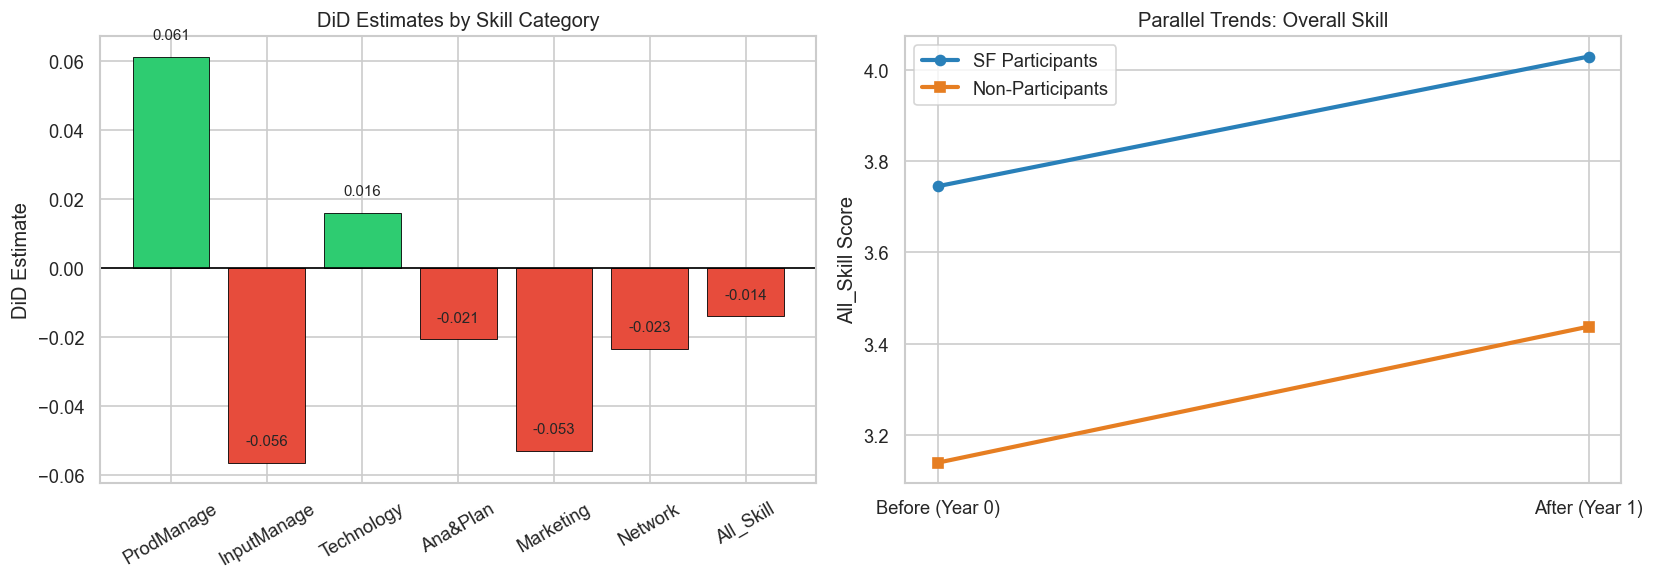
\includegraphics[width=0.8\textwidth]{images/fig_DiD.png}
\caption{แนวโน้มคะแนนทักษะเฉลี่ยของเกษตรกรกลุ่มเข้าร่วมโครงการ (SF) และกลุ่มไม่เข้าร่วมโครงการ (Non-SF) ในช่วงก่อนและหลังการดำเนินโครงการ (การตรวจสอบสมมติฐานแนวโน้มขนาน)}
\label{fig:parallel}
\end{figure}

ในขณะเดียวกัน ระดับคะแนนเฉลี่ยของกลุ่ม SF สูงกว่ากลุ่ม Non-SF ตั้งแต่ก่อนเริ่มโครงการ สะท้อนความแตกต่างของคุณลักษณะตั้งต้นและความเป็นไปได้ของการคัดเลือกเข้าร่วมโครงการ (self-selection) ซึ่งเป็นกลไกหนึ่งของ selection bias

ผลดังกล่าวสอดคล้องกับผลการวิเคราะห์เชิงพรรณนาและแบบจำลอง Probit ในหัวข้อ 4.1 ดังนั้น การออกแบบการวิเคราะห์ในงานวิจัยนี้จึงใช้ PSM เพื่อลดความเอนเอียงจาก KNN ก่อนใช้ DID เพื่อหักล้างความแตกต่างคงที่ระหว่างกลุ่ม (time-invariant differences) และผลของเวลา (common shocks) ในการประมาณผลกระทบเฉลี่ยของโครงการ

ทั้งนี้ การตีความผล DID ยังควรพิจารณาควบคู่กับความเป็นไปได้ของปัจจัยที่ไม่สามารถสังเกตได้ (unobserved factors) ซึ่งอาจก่อให้เกิด selection bias ส่วนที่เหลืออยู่

% ---------------- FIGURE 4.2 ----------------
\begin{figure}[ht]
\centering
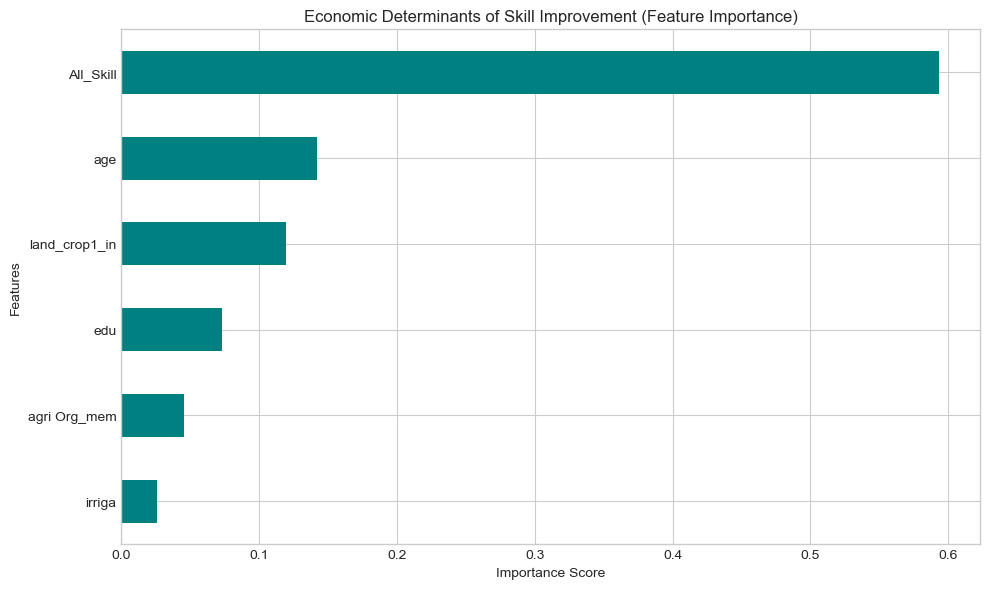
\includegraphics[width=0.7\textwidth]{images/did_compare.png}
\caption{การเปรียบเทียบคะแนนทักษะเฉลี่ยของเกษตรกรกลุ่มเข้าร่วมโครงการ (SF) และกลุ่มไม่เข้าร่วมโครงการ (Non-SF) ระหว่างปี 2565 (ก่อนเข้าร่วม) และปี 2566 (หลังเข้าร่วม)}
\label{fig:did_compare}
\end{figure}

ภาพที่~\ref{fig:did_compare} แสดงให้เห็นว่า คะแนนทักษะเฉลี่ยของกลุ่ม SF สูงกว่ากลุ่ม Non-SF ทั้งก่อนและหลังการดำเนินโครงการ โดยผลต่างระหว่างกลุ่มในปี 2565 และปี 2566 มีขนาดใกล้เคียงกัน สะท้อนว่า “ผลต่างระหว่างกลุ่ม” ไม่ได้เปลี่ยนแปลงอย่างมีนัยสำคัญภายหลังโครงการ

เมื่อพิจารณาร่วมกับสมมติฐานแนวโน้มขนานในภาพที่~\ref{fig:parallel} รูปแบบดังกล่าวสอดคล้องกับผลการประมาณแบบจำลอง DID ในหัวข้อ 4.3 ที่คาดว่าค่าสัมประสิทธิ์ปฏิสัมพันธ์ (Diff-in-Diff) จะมีขนาดเล็กและไม่แตกต่างจากศูนย์ทางสถิติ

กล่าวอีกนัยหนึ่ง การเพิ่มขึ้นของคะแนนในช่วงเวลาดังกล่าวอาจเกิดขึ้นในทั้งสองกลุ่มในทิศทางที่คล้ายกัน มากกว่าจะเป็นผลเฉพาะจากการเข้าร่วมโครงการ

\section{ผลการประเมินผลกระทบของโครงการ (DID Results)}

ภายใต้สมมติฐานแนวโน้มขนานที่ได้รับการสนับสนุนจากหลักฐานเชิงกราฟในหัวข้อ 4.2 (ภาพที่~\ref{fig:parallel}--\ref{fig:did_compare}) ผู้วิจัยประมาณผลกระทบของการเข้าร่วมโครงการต่อคะแนนทักษะรวมของเกษตรกรด้วยวิธี Difference-in-Differences (DID)

โดยสรุปผลการเปรียบเทียบค่าเฉลี่ยก่อนและหลังของกลุ่ม SF และ Non-SF และค่าประมาณผลกระทบสุทธิ (Diff-in-Diff) แสดงไว้ในตารางที่~\ref{tab:did} โดยมีรายละเอียดที่น่าสนใจ ดังต่อไปนี้

\begin{itemize}

\item \textbf{ช่วงก่อนเข้าร่วมโครงการ (ปี 2565)}: ค่าเฉลี่ยคะแนนทักษะรวมของกลุ่ม SF สูงกว่ากลุ่ม Non-SF โดยมีผลต่างเท่ากับ 0.607 และแตกต่างกันอย่างมีนัยสำคัญทางสถิติ

\item \textbf{ช่วงหลังเข้าร่วมโครงการ (ปี 2566)}: ค่าเฉลี่ยคะแนนทักษะรวมของกลุ่ม SF ยังคงสูงกว่ากลุ่ม Non-SF โดยมีผลต่างเท่ากับ 0.602 และแตกต่างกันอย่างมีนัยสำคัญทางสถิติ

\item \textbf{ผลกระทบสุทธิของโครงการ (Diff-in-Diff)}: ค่าสัมประสิทธิ์ Diff-in-Diff เท่ากับ -0.005 และไม่แตกต่างจากศูนย์อย่างมีนัยสำคัญทางสถิติ (p-value = 0.896) สะท้อนว่า การเปลี่ยนแปลงของคะแนนทักษะรวมของกลุ่ม SF ไม่ได้เพิ่มขึ้นมากกว่ากลุ่ม Non-SF ในช่วงเวลาเดียวกัน

\end{itemize}

\begin{table}[ht]
\centering
\small
\setlength{\tabcolsep}{4pt}
\renewcommand{\arraystretch}{1.1}

\caption{ผลการประเมินผลกระทบของโครงการต่อทักษะเกษตรกรด้วยวิธีผลต่างของผลต่าง (Difference-in-Differences: DID)}
\label{tab:did}

\begin{tabular}{lcccc}
\hline
\textbf{Outcome: All farm skills} & \textbf{Mean} & \textbf{Difference} & \textbf{S.E.} & \textbf{p-value} \\
\hline

\multicolumn{5}{l}{\textbf{ปี 2565 (ก่อนเข้าร่วม)}} \\
กลุ่มที่ไม่เข้าร่วม (Non-SF) & 3.130 & & & \\
กลุ่มที่เข้าร่วม (SF) & 3.737 & & & \\
ผลต่างก่อนเริ่ม (Diff) & & 0.607 & 0.063 & 0.000$^{***}$ \\

\multicolumn{5}{l}{\textbf{ปี 2566 (หลังเข้าร่วม)}} \\
กลุ่มที่ไม่เข้าร่วม (Non-SF) & 3.423 & & & \\
กลุ่มที่เข้าร่วม (SF) & 4.025 & & & \\
ผลต่างหลังจบ (Diff) & & 0.602 & 0.063 & 0.000$^{***}$ \\

\textbf{ผลกระทบสุทธิ (Diff-in-Diff)} & & -0.005 & 0.090 & 0.896 \\

\hline
\end{tabular}
\end{table}

กล่าวโดยสรุป จากผลการทดลองข้างต้นสามารถที่จะตอบคำถามวัตถุประสงค์การวิจัยข้อที่ 1 ซึ่งมุ่งประเมินผลกระทบของการเข้าร่วมโครงการเกษตรกรอัจฉริยะต่อทักษะของเกษตรกร 
พบว่า แม้กลุ่ม SF จะมีระดับคะแนนทักษะรวมสูงกว่ากลุ่ม Non-SF ทั้งก่อนและหลังการดำเนินโครงการ แต่เมื่อควบคุมความแตกต่างคงที่ระหว่างกลุ่มและผลของเวลาด้วยวิธี DID แล้ว 
ไม่พบหลักฐานเชิงประจักษ์ว่าการเข้าร่วมโครงการส่งผลให้คะแนนทักษะรวมเพิ่มขึ้นมากกว่ากลุ่มที่ไม่เข้าร่วมอย่างมีนัยสำคัญทางสถิติ ตามผลการประมาณในตารางที่~\ref{tab:did}

ทั้งนี้ ผลการวิเคราะห์ในระดับมิติทักษะชี้ว่า ค่าประมาณ Diff-in-Diff ของทักษะด้านการจัดการการผลิต (ProdManage) และทักษะด้านเทคโนโลยี (Technology) เป็นบวก
 (+0.061 และ +0.016 ตามลำดับ) แต่มีขนาดผลกระทบค่อนข้างเล็ก จึงยังไม่อาจสรุปได้ว่ามีการพัฒนาทักษะที่เด่นชัดจากการเข้าร่วมโครงการ

ภายใต้ข้อจำกัดของข้อมูลและความเป็นไปได้ของปัจจัยที่ไม่สามารถสังเกตได้ (unobserved factors) ที่อาจมีผลต่อการเข้าร่วม 
(ดังที่อภิปรายในหัวข้อ 4.1--4.2) ผลดังกล่าวสะท้อนความจำเป็นในการพิจารณา (1) การออกแบบเนื้อหาและความเข้มข้นของการอบรม
ให้สอดคล้องกับระดับพื้นฐานของผู้เข้าร่วม และ (2) การกำหนดกลุ่มเป้าหมายและมาตรการสนับสนุนร่วม เช่น โครงสร้างพื้นฐานและการเข้าถึงเทคโนโลยี เพื่อเพิ่มโอกาสที่โครงการจะก่อให้เกิดผลลัพธ์ด้านทักษะอย่างมีนัยสำคัญ

จากข้อค้นพบข้างต้น ขั้นตอนถัดไปจึงมุ่งพิจารณาหลักฐานสนับสนุนที่ช่วยอธิบายกลไกและความแตกต่างของผลลัพธ์ระหว่างเกษตรกรรายบุคคล 
โดยเริ่มจากการสำรวจโครงสร้างความสัมพันธ์ของมิติทักษะในหัวข้อ~4.4 และต่อยอดด้วยการวิเคราะห์เชิงพยากรณ์ด้วยการเรียนรู้ของเครื่อง และการอธิบายแบบจำลองด้วย SHAP ในหัวข้อ~4.5--4.6 เพื่อทำความเข้าใจความไม่เป็นเนื้อเดียวกันของผลลัพธ์อาจถูกกลบเมื่อพิจารณาในระดับค่าเฉลี่ยจาก DID

\section{การวิเคราะห์ความสัมพันธ์ของทักษะ (Correlation Analysis)}

หัวข้อ 4.4 มีวัตถุประสงค์เพื่อสำรวจ “ความเชื่อมโยงระหว่างมิติทักษะ” ของเกษตรกร โดยใช้การวิเคราะห์สหสัมพันธ์ (correlation analysis) เพื่อทำความเข้าใจว่า ทักษะแต่ละมิติมีความสัมพันธ์เกื้อหนุนกันในลักษณะใด

ผลการวิเคราะห์ถูกนำเสนอในรูปแบบตารางความสัมพันธ์ (correlation table) เพื่อสะท้อนภาพรวมของโครงสร้างทักษะ และใช้เป็นหลักฐานประกอบในการอธิบายว่าเหตุใดผลกระทบเฉลี่ยจากการประเมินเชิงสาเหตุในหัวข้อ 4.3 อาจไม่ปรากฏเด่นชัด หากการพัฒนาทักษะมีลักษณะพึ่งพาปัจจัยหลายด้านและมีความแตกต่างระหว่างรายบุคคล (heterogeneity)

% -------- FIGURE 4.3 --------
\begin{figure}[htbp]
\centering
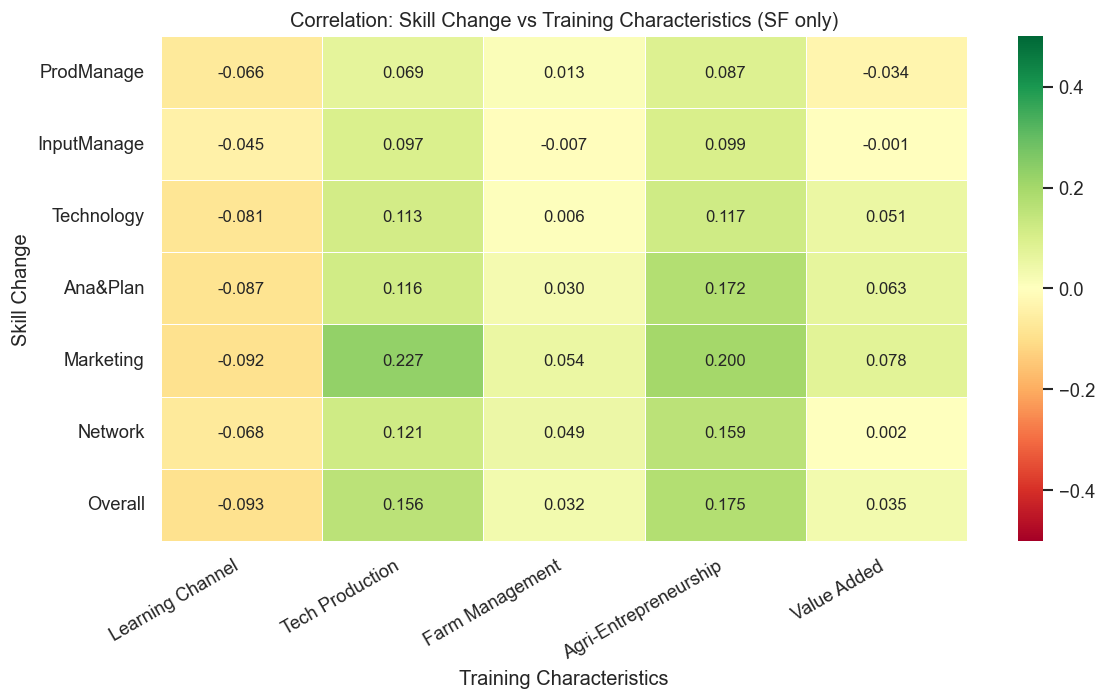
\includegraphics[width=0.9\textwidth]{images/fig_Correlation.png}
\caption{ความสัมพันธ์ระหว่างมิติทักษะของเกษตรกร (Correlation Network)}
\label{fig:corr}
\end{figure}

ภาพที่~\ref{fig:corr} แสดงเครือข่ายความสัมพันธ์เชิงสหสัมพันธ์ระหว่างมิติทักษะ โดยสามารถสรุปสาระสำคัญได้ ดังนี้

\begin{itemize}

\item มิติทักษะมีความเชื่อมโยงกันสะท้อนว่า การพัฒนาทักษะในมิติหนึ่งมีแนวโน้มสัมพันธ์กับการเปลี่ยนแปลงของทักษะในมิติอื่นร่วมด้วย

\item นัยเชิงนโยบาย คือ การยกระดับทักษะควรออกแบบแบบบูรณาการ โดยดำเนินควบคู่กับการเสริมปัจจัยเอื้อด้านทุนมนุษย์ ทรัพยากร และโครงสร้างพื้นฐาน มากกว่าการมุ่งเน้นการอบรมเพียงองค์ประกอบเดียว

\end{itemize}

ในภาพรวม การที่มิติทักษะเชื่อมโยงกันเป็นเครือข่ายสะท้อนว่า “การเพิ่มขึ้นของทักษะรวม” อาจต้องอาศัยองค์ประกอบหลายด้านควบคู่กัน ทั้งด้านความรู้ การจัดการ เทคโนโลยี ตลอดจนปัจจัยเอื้อด้านทรัพยากรและโครงสร้างพื้นฐาน

อีกทั้งเมื่อเกษตรกรมีระดับความพร้อมแตกต่างกัน ผลลัพธ์จากการเข้าร่วมโครงการจึงอาจกระจายไม่เท่ากันระหว่างรายบุคคล (heterogeneous effects) และทำให้ค่าประมาณผลกระทบเฉลี่ยด้วย DID ในหัวข้อ 4.3 ไม่ปรากฏเด่นชัดในภาพรวม

ดังนั้น ในหัวข้อ 4.5 ผู้วิจัยจึงประยุกต์ใช้การเรียนรู้ของเครื่อง (machine learning) เพื่อพยากรณ์การเปลี่ยนแปลงทักษะและระบุปัจจัยสำคัญที่สัมพันธ์กับผลลัพธ์ดังกล่าว

\section{การพัฒนาแบบจำลองการเรียนรู้ของเครื่องเพื่อพยากรณ์การเปลี่ยนแปลงทักษะ (Machine Learning Model)}

หัวข้อ 4.5 นำเสนอขั้นตอนการพัฒนาแบบจำลองการเรียนรู้ของเครื่อง (machine learning) เพื่อพยากรณ์การเปลี่ยนแปลงทักษะของเกษตรกร และสรุปผลการประเมินความสำคัญของตัวแปร (feature importance) เพื่อระบุปัจจัยที่สัมพันธ์กับผลลัพธ์ในเชิงพยากรณ์ โดยผลในภาพที่~\ref{fig:importance} ชี้ว่า ปัจจัยด้านทุนมนุษย์และทรัพยากร/โครงสร้างพื้นฐานของฟาร์มมีบทบาทต่อการพยากรณ์การเปลี่ยนแปลงทักษะมากกว่าตัวแปรที่สะท้อนการอบรมเพียงอย่างเดียว โดยพบข้อสรุปที่น่าสนใจ ดังต่อไปนี้

\begin{itemize}

\item \textbf{บทบาทของทักษะตั้งต้น:} ตัวแปรที่เกี่ยวข้องกับทักษะด้านเทคโนโลยี/ดิจิทัลและระดับทักษะตั้งต้น (baseline skills) ปรากฏเป็นตัวทำนายสำคัญของการเปลี่ยนแปลงทักษะ

\item \textbf{บทบาทของทุนมนุษย์และทรัพยากร:} ปัจจัยเชิงประชากรและทรัพยากรการผลิต (เช่น อายุ ระดับการศึกษา และขนาดพื้นที่ถือครอง) มีส่วนช่วยอธิบายความแตกต่างของผลลัพธ์ระหว่างเกษตรกรรายบุคคล

\end{itemize}

% -------- FIGURE 4.4 --------
\begin{figure}[htbp]
\centering
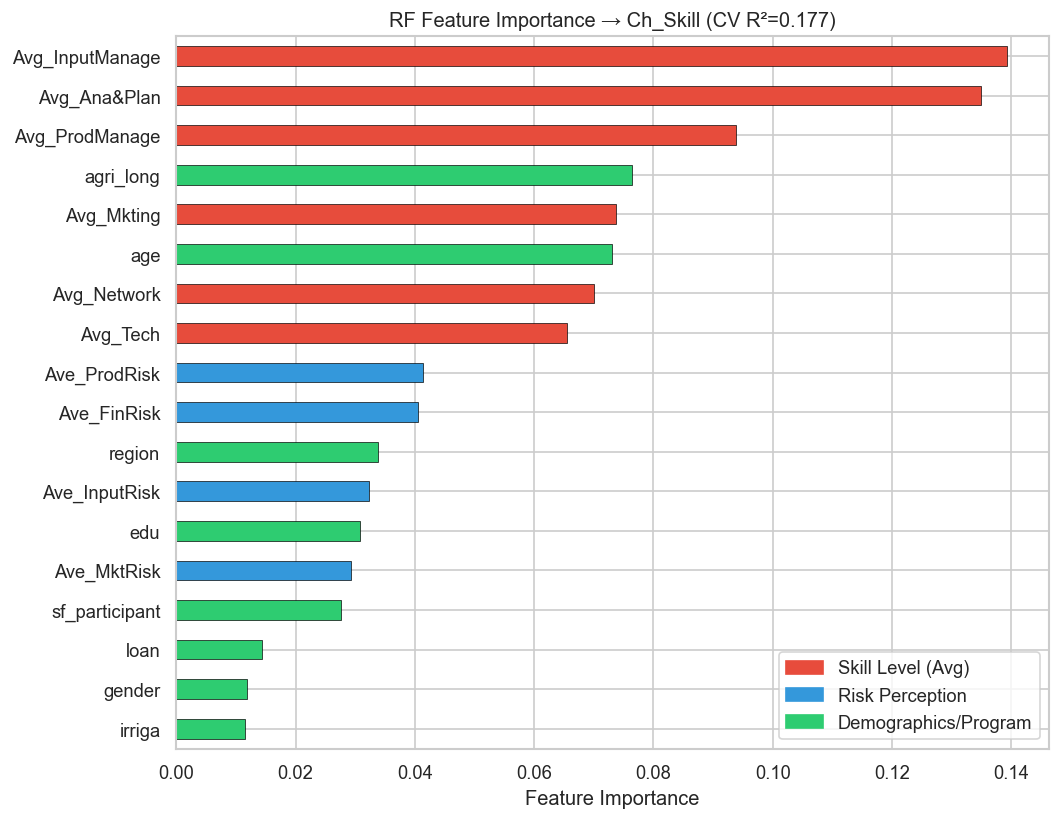
\includegraphics[width=0.85\textwidth]{images/fig_FeatureImportance.png}
\caption{ความสำคัญของตัวแปรที่สัมพันธ์กับการเปลี่ยนแปลงทักษะ (Feature Importance)}
\label{fig:importance}
\end{figure}

ทั้งนี้ การวิเคราะห์ feature importance จะช่วยให้สามารถระบุได้ว่า ``ตัวแปรใดสำคัญ'' ต่อการพยากรณ์ แต่ยังไม่สามารถอธิบายได้ว่า ตัวแปรดังกล่าวส่งผลต่อการเปลี่ยนแปลงทักษะในทิศทางใด และแตกต่างกันระหว่างรายบุคคลอย่างไร ดังนั้น หัวข้อ 4.6 จึงใช้เทคนิค SHAP เพื่ออธิบายอิทธิพลของตัวแปรในระดับรายบุคคลอย่างละเอียด

\section{การอธิบายผลด้วยวิธี SHAP}

เพื่อเพิ่มความสามารถในการตีความผลการพยากรณ์จากแบบจำลองการเรียนรู้ของเครื่องในหัวข้อ 4.5 ผู้วิจัยประยุกต์ใช้เทคนิค SHAP (SHapley Additive exPlanations) ซึ่งช่วยอธิบาย “ทิศทาง” และ “ขนาด” ของอิทธิพลของตัวแปรต่อค่าที่แบบจำลองพยากรณ์ในระดับรายบุคคล กล่าวคือ สามารถระบุได้ว่าตัวแปรหนึ่ง ๆ มีแนวโน้มเพิ่มหรือลดค่าพยากรณ์ และมีอิทธิพลมากน้อยเพียงใด เมื่อเทียบกับตัวแปรอื่น

ภาพที่~\ref{fig:shap_summary} เป็นผลการอธิบายแบบจำลองด้วย SHAP ในภาพรวม (summary) เพื่อตอบคำถามที่ว่า “ใครมีอิทธิพลต่อ model มากที่สุด โดยไม่สนทิศทาง” ข้อค้นพบที่สำคัญที่สุดคือ Avg Mkting มีค่าสูงกว่าตัวอื่นเกือบสามเท่า (0.22 เทียบกับ 0.083) ซึ่งหมายความว่า ระดับทักษะ Marketing ที่เกษตรกรมีอยู่ก่อนเข้าโครงการ เป็นตัวทำนาย Ch\_Skill ที่ทรงพลังที่สุด มากกว่าหลักสูตรทุกตัวรวมกัน

% -------- FIGURE 4.5 --------
\begin{figure}[htbp]
\centering
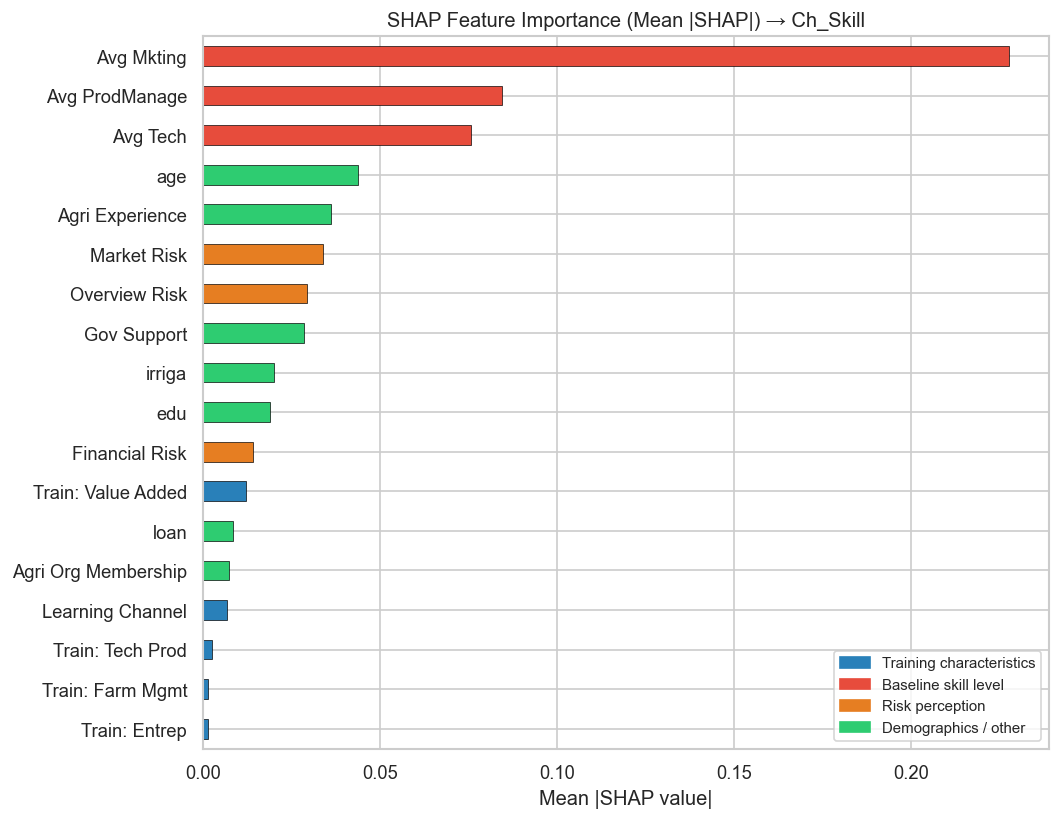
\includegraphics[width=0.85\textwidth]{images/fig_SHAP_Bar.png}
\caption{ผลการอธิบายตัวแปรด้วย SHAP (สรุปภาพรวม)}
\label{fig:shap_summary}
\end{figure}

ภาพที่~\ref{fig:shap_detail} แสดงการกระจายของค่าอิทธิพล SHAP รายตัวแปร ซึ่งช่วยให้เห็นความแปรปรวนของอิทธิพลในระดับรายบุคคล (heterogeneity) กล่าวคือ ตัวแปรเดียวกันอาจมีอิทธิพลต่อเกษตรกรแต่ละรายแตกต่างกันตามระดับค่าและบริบทของแต่ละราย

ช่วยทำให้เห็นว่า ปัจจัยเดิมชุดเดียวกันอาจมีบทบาทต่อการพยากรณ์การเปลี่ยนแปลงทักษะไม่เท่ากัน ซึ่งสนับสนุนข้อค้นพบเชิงภาพรวมในหัวข้อ 4.3 ที่ค่าประมาณผลกระทบเฉลี่ยจาก DID ไม่เด่นชัด

โดยมีข้อค้นพบสำคัญ คือ ค่า Avg Mkting มี pattern แบบ "V กลับ" คือ จุดสีน้ำเงิน (Mkting เดิมต่ำ) กระจายไปทางขวา และจุดสีแดง (Mkting เดิมสูง) กระจายไปทางซ้าย โดยการกระจายตัวลักษณะนี้เรียกว่า Regression to the Mean หมายถึง คนที่เก่งอยู่แล้วพัฒนาได้ยาก ส่วนคนที่ยังอ่อนกลับมีพื้นที่เติบโตมากกว่า

% -------- FIGURE 4.6 --------
\begin{figure}[htbp]
\centering
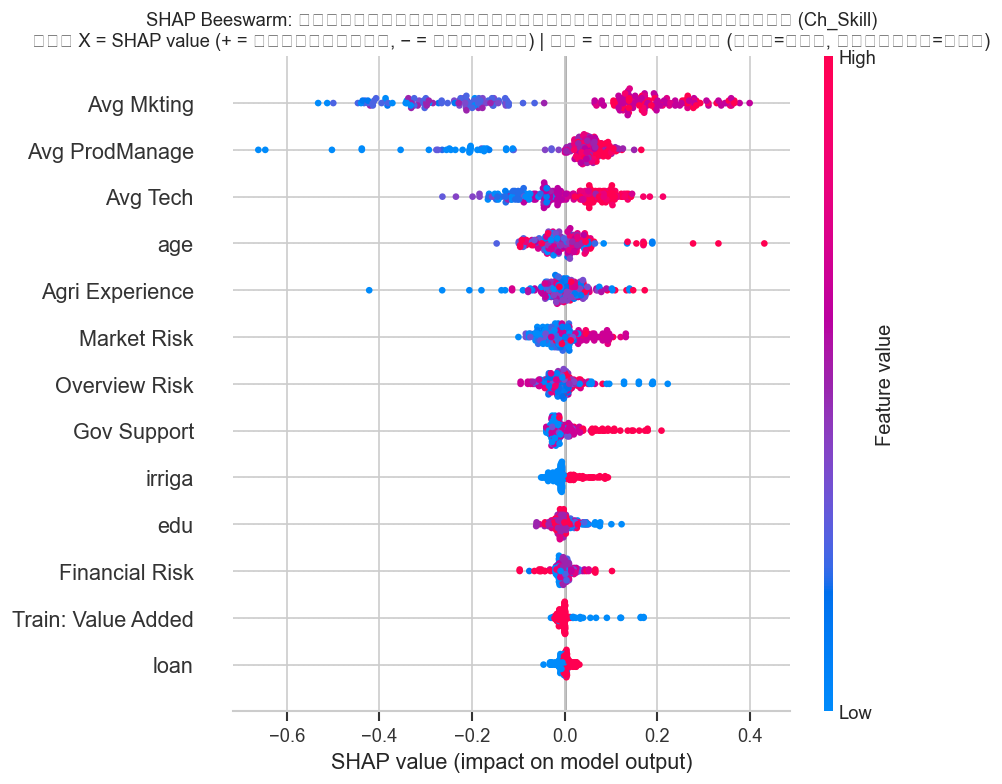
\includegraphics[width=0.85\textwidth]{images/fig_SHAP_Beeswarm.png}
\caption{ผลการอธิบายตัวแปรด้วย SHAP (รายตัวแปร)}
\label{fig:shap_detail}
\end{figure}

ทั้งนี้ ผล SHAP มีวัตถุประสงค์เพื่อการอธิบายเชิงพยากรณ์และการทำความเข้าใจรูปแบบความสัมพันธ์ในข้อมูล จึงไม่ควรถูกตีความเป็นความสัมพันธ์เชิงเหตุและผลโดยตรง

จากผลการอธิบายแบบจำลองในระดับรายบุคคลดังกล่าว พบว่า โครงการ SF ส่งผลต่อทักษะ แต่ขนาดผลขึ้นอยู่กับว่าเกษตรกรคนนั้นมีพื้นฐานความรู้แบบไหนมากกว่าหลักสูตรที่เข้าร่วมเรียน

โดยขั้นตอนถัดไปจึงนำปัจจัยสำคัญที่สะท้อนความแตกต่างระหว่างรายบุคคลไปสังเคราะห์ในระดับ “กลุ่ม” ด้วยการวิเคราะห์การจัดกลุ่ม (clustering) เพื่อจำแนกเกษตรกรตามรูปแบบความพร้อมและข้อจำกัดที่คล้ายคลึงกัน ดังนำเสนอในหัวข้อ 4.7

\section{การจำแนกกลุ่มเกษตรกร (Clustering Analysis)}

ผลการอธิบายแบบจำลองด้วย SHAP ในหัวข้อ 4.6 ชี้ให้เห็นว่า ปัจจัยที่สัมพันธ์กับการเปลี่ยนแปลงทักษะมีความแตกต่างกันระหว่างเกษตรกรรายบุคคล สะท้อนลักษณะความไม่เป็นเนื้อเดียวกันของผลลัพธ์ (heterogeneity)

ดังนั้น หัวข้อ 4.7 จึงประยุกต์ใช้การวิเคราะห์การจัดกลุ่ม (clustering) เพื่อจำแนกเกษตรกรตามรูปแบบของศักยภาพและข้อจำกัดที่คล้ายคลึงกัน เพื่อสนับสนุนการตีความผลในระดับกลุ่มย่อยและการออกแบบมาตรการแบบจำเพาะกลุ่มในหัวข้อถัดไป

โดยจากกราฟ PCA พบว่า องค์ประกอบหลักที่หนึ่ง (PC1) สามารถอธิบายความแปรปรวนของข้อมูลได้ 33.1\% และองค์ประกอบหลักที่สอง (PC2) อธิบายได้ 17.1\% รวมกันเป็น 50.2\% ของความแปรปรวนทั้งหมด

ซึ่งถือว่าสามารถสะท้อนโครงสร้างหลักของข้อมูลได้ในระดับหนึ่ง และเมื่อพิจารณากราฟฝั่งซ้าย (Farmer Clusters) ซึ่งใช้วิธี k-means (k=2) ในการแบ่งกลุ่ม พบว่า การจัดกลุ่มมีลักษณะการแยกตัวตามแกน PC1 อย่างชัดเจน

อย่างไรก็ตาม จุดข้อมูลของทั้งสองกลุ่มยังมีพื้นที่ทับซ้อนกันบริเวณค่ากลางของ PC1 ค่อนข้างมาก สะท้อนว่าการแบ่งกลุ่มดังกล่าวไม่ได้มีความชัดเจนสูง ซึ่งสอดคล้องกับค่า silhouette score ที่อยู่ในระดับต่ำ

แสดงให้เห็นว่าข้อมูลมีลักษณะเป็นความต่อเนื่อง (continuum) มากกว่าการแบ่งออกเป็นกลุ่มที่แยกจากกันชัดเจน

ในเชิงการตีความเชิงเนื้อหา PC1 น่าจะสะท้อนถึง “ระดับทักษะหรือศักยภาพโดยรวมของเกษตรกร” กล่าวคือ เกษตรกรที่มีค่า PC1 สูงมีแนวโน้มที่จะมีทักษะสูงกว่า ในขณะที่ค่า PC1 ต่ำสะท้อนระดับทักษะที่ต่ำกว่า

% -------- FIGURE 4.7 --------
\begin{figure}[htbp]
\centering
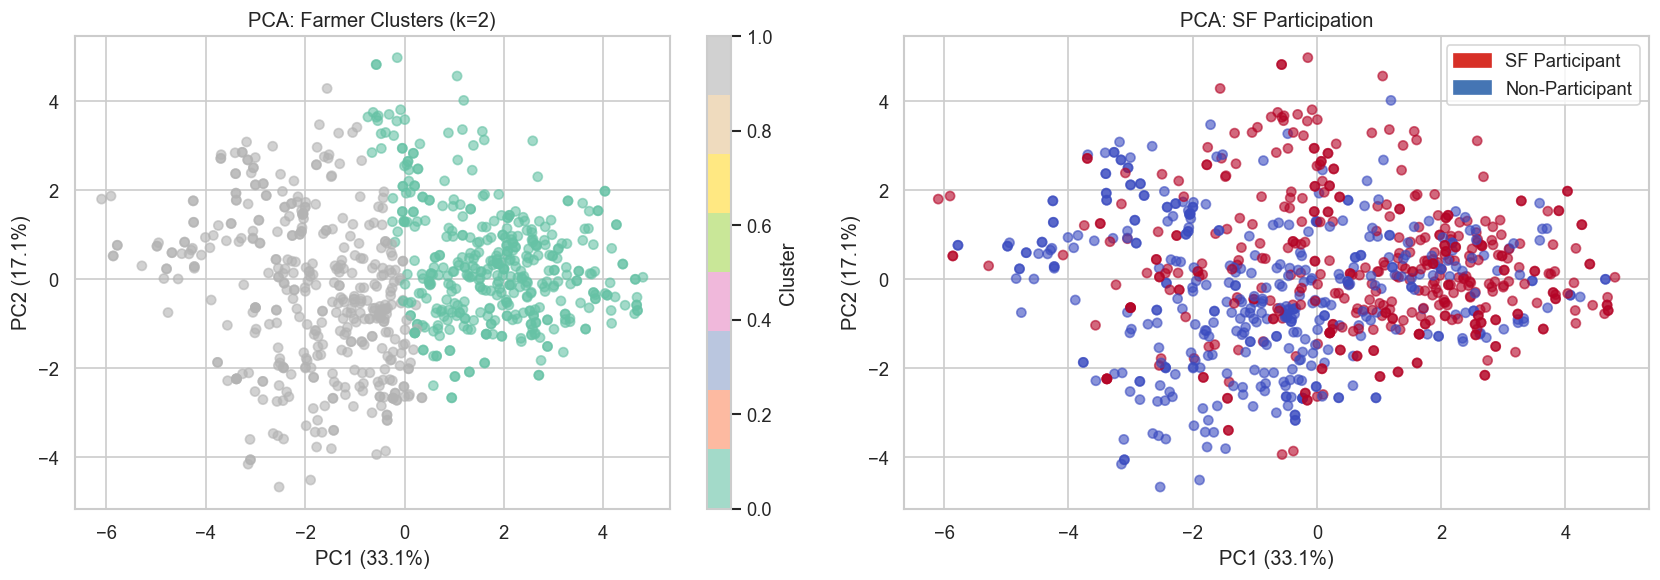
\includegraphics[width=0.9\textwidth]{images/fig_PCA.png}
\caption{ผลการจัดกลุ่มเกษตรกรด้วยการวิเคราะห์การจัดกลุ่ม (Clustering) (ภาพรวม)}
\label{fig:cluster_overview}
\end{figure}

อย่างไรก็ตาม จากผลการวิเคราะห์พบประเด็นวิกฤติที่สำคัญ ดังแสดงในภาพที่~\ref{fig:cluster_detail} คือ กลุ่มเกษตรกรที่มีระดับทักษะต่ำ (Cluster 1) มีค่าการเปลี่ยนแปลงของทักษะ (Ch\_Skill) เป็นลบ (−0.26) สะท้อนว่าทักษะลดลงหลังเข้าร่วมโครงการ

ซึ่งชี้ให้เห็นถึงผลกระทบเชิงลบของการดำเนินโครงการในบางกลุ่ม และเมื่อเชื่อมโยงกับผลการวิเคราะห์ SHAP พบว่าเป็นลักษณะของ ceiling effect มากกว่าการเกิด floor effect กล่าวคือ โครงการให้ประโยชน์กับผู้ที่มีทักษะสูงอยู่แล้ว

ขณะที่ผู้มีทักษะต่ำไม่สามารถรับเนื้อหาได้อย่างมีประสิทธิภาพ ส่งผลให้เกิดความเหลื่อมล้ำในการพัฒนา และอาจนำไปสู่การออกแบบนโยบายที่ไม่สอดคล้องกับศักยภาพของผู้เข้าร่วม

% -------- FIGURE 4.8 --------
\begin{figure}[htbp]
\centering
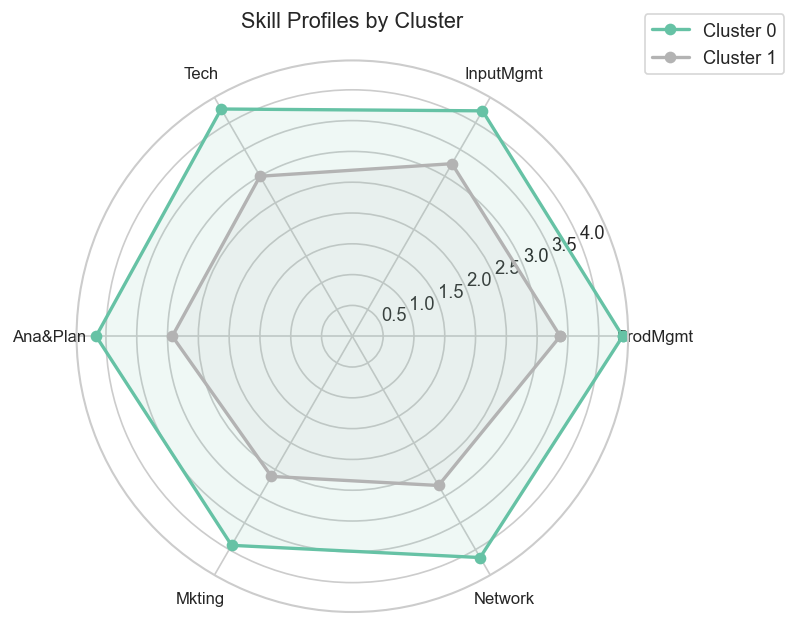
\includegraphics[width=0.9\textwidth]{images/fig_RadarCluster.png}
\caption{ผลการจัดกลุ่มเกษตรกรด้วยการวิเคราะห์การจัดกลุ่ม (Clustering) (รายละเอียดจำแนกกลุ่ม)}
\label{fig:cluster_detail}
\end{figure}

จากผลการวิเคราะห์การจัดกลุ่มในภาพที่~\ref{fig:cluster_overview}--\ref{fig:cluster_detail} สามารถจำแนกเกษตรกรออกเป็น 2 กลุ่มหลักตามรูปแบบความพร้อมด้านทักษะและปัจจัยสนับสนุนด้านทรัพยากร/โครงสร้างพื้นฐาน ประกอบไปด้วย กลุ่มเกษตรกรศักยภาพสูงและกลุ่มเกษตรที่มีข้อจำกัดเชิงโครงสร้าง

การจำแนกดังกล่าวช่วยเติมเต็มข้อค้นพบในหัวข้อ 4.3–4.6 กล่าวคือ แม้การประเมินผลเชิงสาเหตุด้วย DID ไม่พบผลกระทบเฉลี่ยของโครงการต่อทักษะรวมอย่างมีนัยสำคัญ แต่หลักฐานเชิงพยากรณ์จากการเรียนรู้ของเครื่องและ SHAP ชี้ว่า ปัจจัยด้านทุนมนุษย์ ทักษะตั้งต้น และทรัพยากร/โครงสร้างพื้นฐานมีบทบาทต่อการเปลี่ยนแปลงทักษะและมีความแตกต่างระหว่างรายบุคคล

ดังนั้น การจำแนกกลุ่มจึงช่วยทำให้ภาพของความแตกต่างเชิงโครงสร้างดังกล่าวชัดเจนขึ้นในระดับกลุ่มย่อย

\textbf{กลุ่มที่ 1: กลุ่มศักยภาพสูง (High-Potential)}

เป็นกลุ่มที่มีระดับทักษะตั้งต้นค่อนข้างสูงและมีความพร้อมด้านทรัพยากรการผลิตมากกว่าเมื่อเทียบกับอีกกลุ่มหนึ่ง ซึ่งสะท้อน “ขีดความสามารถในการดูดซับความรู้” (absorptive capacity) ที่สูงกว่า

\begin{itemize}
\item ทักษะตั้งต้น: ระดับทักษะเดิมและองค์ประกอบด้านเทคโนโลยีอยู่ในระดับสูงกว่าค่าเฉลี่ย
\item ทรัพยากรสนับสนุน: มีความพร้อมด้านทรัพยากร เช่น การเข้าถึงโครงสร้างพื้นฐานบางด้าน
\end{itemize}

\textbf{กลุ่มที่ 2: กลุ่มมีข้อจำกัดเชิงโครงสร้าง (Constraint Group)}

เป็นกลุ่มที่มีระดับทักษะตั้งต้นต่ำและมีข้อจำกัดด้านทรัพยากรและโครงสร้างพื้นฐาน

\begin{itemize}
\item ทักษะตั้งต้น: ระดับทักษะเดิมอยู่ในระดับต่ำ
\item ข้อจำกัดเชิงโครงสร้าง: มีข้อจำกัดด้านทรัพยากร เช่น การเข้าถึงระบบชลประทาน
\end{itemize}

การวิเคราะห์เชิงลึกด้วย SHAP dependence plot แสดงให้เห็นว่า การเข้าร่วมโครงการ SF มีผลในการลดความแปรปรวนของผลลัพธ์ (variance reduction) โดยกลุ่มผู้เข้าร่วมมีการกระจายของค่า SHAP แคบลง

อย่างไรก็ตาม การลดความแปรปรวนดังกล่าวไม่ได้มาพร้อมกับการเพิ่มขึ้นของค่าผลลัพธ์โดยเฉลี่ยอย่างสม่ำเสมอ สะท้อนว่าโครงการทำหน้าที่เป็นกลไกเชิงมาตรฐาน (standardization mechanism) มากกว่าการยกระดับศักยภาพ

และที่สำคัญที่สุด ผลการวิเคราะห์ SHAP รายกลุ่มพบว่า ตัวแปรการเข้าร่วม SF มีอิทธิพลต่อการทำนายการเปลี่ยนแปลงทักษะ (Ch\_Skill) ในกลุ่มทักษะต่ำ (Cluster 1) สูงกว่ากลุ่มทักษะสูง

อย่างไรก็ตาม เมื่อพิจารณาร่วมกับค่าผลลัพธ์จริงที่ Cluster 1 มีค่า Ch\_Skill เป็นลบ (−0.26) ข้อค้นพบนี้ชี้ให้เห็นว่า โครงการ SF อาจส่งผลกระทบเชิงลบต่อกลุ่มเปราะบางโดยไม่ได้ตั้งใจ

ซึ่งสะท้อนถึงความจำเป็นในการออกแบบมาตรการแบบจำแนกกลุ่ม (targeted intervention) หรือการจัดหลักสูตรตามระดับศักยภาพ (tiered training design)

\section{กรอบนโยบายเชิงข้อเสนอ (Policy Framework – AI-Driven)}

หัวข้อ 4.8 นำเสนอกรอบข้อเสนอเชิงนโยบายเพื่อสนับสนุนการพัฒนาทักษะของเกษตรกร โดยยึดโยงกับหลักฐานเชิงประจักษ์จากหัวข้อ 4.1–4.7 อย่างเป็นระบบ กล่าวคือ ผลการประเมินเชิงสาเหตุด้วย DID (หัวข้อ 4.3) ไม่พบผลกระทบเฉลี่ยของโครงการต่อคะแนนทักษะรวมอย่างมีนัยสำคัญ

ขณะที่หลักฐานจากการวิเคราะห์ความสัมพันธ์ การพยากรณ์ด้วยการเรียนรู้ของเครื่อง และการอธิบายแบบจำลองด้วย SHAP ตลอดจนผลการจำแนกกลุ่ม (หัวข้อ 4.4–4.7) ชี้ว่า การเปลี่ยนแปลงทักษะมีความไม่เป็นเนื้อเดียวกัน (heterogeneity) และสัมพันธ์กับความพร้อมตั้งต้นด้านทุนมนุษย์และทรัพยากร/โครงสร้างพื้นฐาน

ดังนั้น กรอบนโยบายในส่วนนี้จึงมุ่งเสนอแนวทางการออกแบบมาตรการแบบจำเพาะกลุ่ม (targeted approach) เพื่อเพิ่มความสอดคล้องระหว่างรูปแบบการสนับสนุนกับข้อจำกัดและศักยภาพของผู้รับนโยบาย

ทั้งนี้ การสกัดกฎเกณฑ์เชิงตรรกะจากแบบจำลองต้นไม้ตัดสินใจ (decision tree) ถูกนำมาใช้เพื่อสื่อสารเกณฑ์การจำแนกกลุ่มในรูปแบบที่เข้าใจง่าย และสนับสนุนการกำหนดกลุ่มเป้าหมายเชิงปฏิบัติการ โดยกฎดังกล่าวสะท้อนความสัมพันธ์เชิงพยากรณ์ภายใต้ชุดข้อมูลที่ศึกษา มิใช่ข้อสรุปเชิงเหตุและผลโดยตรง

อีกทั้งควรพิจารณาควบคู่กับความเป็นไปได้ของ selection bias (ทั้งจากตัวแปรที่สังเกตได้และไม่สังเกตได้) ที่อาจมีอยู่ในการคัดเลือกผู้เข้าร่วมและในการสังเกตผลลัพธ์

\begin{enumerate}

\item \textbf{กลุ่มศักยภาพสูงเพื่อการต่อยอด (High-Potential Strategy)}

\begin{itemize}
\item \textbf{เกณฑ์การกำหนดกลุ่ม:} เกษตรกรที่มีความพร้อมด้านทรัพยากรการผลิต/โครงสร้างพื้นฐาน เช่น การเข้าถึงระบบชลประทาน และมีระดับทักษะเดิมอยู่ในระดับปานกลางถึงสูง

\item \textbf{หลักฐานสนับสนุน:} ผลการพยากรณ์และการอธิบายแบบจำลอง (หัวข้อ 4.5–4.6) ชี้บทบาทของระดับทักษะตั้งต้นและตัวแปรด้านทรัพยากรต่อการเปลี่ยนแปลงทักษะ และผลการจำแนกกลุ่ม (หัวข้อ 4.7) สนับสนุนว่ากลุ่มนี้มีขีดความสามารถในการดูดซับความรู้สูงกว่าโดยเปรียบเทียบ

\item \textbf{ข้อเสนอเชิงนโยบาย:} จัดกิจกรรมพัฒนาทักษะขั้นสูงเพื่อการต่อยอด เช่น การประยุกต์ใช้เซนเซอร์ ระบบควบคุมการให้น้ำ หรือการวิเคราะห์ข้อมูลผลผลิตและตลาด ควบคู่กับการติดตามสนับสนุนเชิงปฏิบัติ (coaching) เพื่อเพิ่มการนำไปใช้จริงและการขยายผลในพื้นที่

\end{itemize}

\item \textbf{กลุ่มพัฒนาทุนมนุษย์และทักษะดิจิทัลเบื้องต้น (Digital Literacy \& Mindset Strategy)}

\begin{itemize}
\item \textbf{เกณฑ์การกำหนดกลุ่ม:} เกษตรกรที่มีความพร้อมด้านทรัพยากรบางส่วน แต่มีข้อจำกัดด้านทุนมนุษย์ เช่น ระดับการศึกษาต่ำ หรือมีทักษะด้านเทคโนโลยีอยู่ในระดับต่ำ

\item \textbf{หลักฐานสนับสนุน:} ผลเชิงพรรณนา (หัวข้อ 4.1) สะท้อนความแตกต่างด้านการศึกษาและทักษะตั้งต้น ขณะที่ผลเชิงพยากรณ์และ SHAP (หัวข้อ 4.5–4.6) ชี้บทบาทของทักษะด้านเทคโนโลยี/ดิจิทัลและระดับทักษะตั้งต้น

\item \textbf{ข้อเสนอเชิงนโยบาย:} จัดโปรแกรมพัฒนาทักษะดิจิทัลสำหรับผู้เริ่มต้น โดยเน้นการเรียนรู้แบบลงมือปฏิบัติ การใช้เครื่องมือที่ไม่ซับซ้อน และการสนับสนุนพี่เลี้ยงในพื้นที่ ก่อนเชื่อมต่อสู่เนื้อหาขั้นสูงในระยะถัดไป

\end{itemize}

\item \textbf{กลุ่มลดคอขวดด้านโครงสร้างพื้นฐาน (Infrastructure-First Strategy)}

\begin{itemize}
\item \textbf{เกณฑ์การกำหนดกลุ่ม:} เกษตรกรที่ไม่สามารถเข้าถึงระบบชลประทาน หรือมีข้อจำกัดด้านโครงสร้างพื้นฐานการผลิตที่สำคัญ

\item \textbf{หลักฐานสนับสนุน:} ผลเชิงพรรณนา (หัวข้อ 4.1) ชี้ว่าเกษตรกรส่วนใหญ่ยังไม่สามารถเข้าถึงระบบชลประทาน และผลการจำแนกกลุ่ม (หัวข้อ 4.7) สะท้อนว่ากลุ่มที่มีข้อจำกัดเชิงโครงสร้างมีความพร้อมด้านทักษะและทรัพยากรต่ำกว่า

\item \textbf{ข้อเสนอเชิงนโยบาย:} จัดลำดับความสำคัญของมาตรการลดคอขวดด้านโครงสร้างพื้นฐาน เช่น การพัฒนาแหล่งน้ำ การเข้าถึงบริการสนับสนุนการผลิต และกลไกประกันความเสี่ยง ควบคู่กับการอบรมทักษะพื้นฐานเพื่อเพิ่มโอกาสในการนำความรู้ไปใช้จริง

\end{itemize}

\end{enumerate}

อนึ่ง กฎการจำแนกกลุ่มจากแบบจำลอง เช่น decision tree มีสถานะเป็น “กรอบสนับสนุนการตัดสินใจ” มิใช่เกณฑ์เชิงนโยบายที่ตายตัว เนื่องจากเป็นความสัมพันธ์เชิงพยากรณ์ภายใต้ข้อมูลที่ศึกษา

ดังนั้น การนำกรอบนโยบายไปใช้ควรดำเนินควบคู่กับการตรวจสอบข้อมูลภาคสนาม การกำหนดตัวชี้วัดผลลัพธ์ที่ชัดเจน และการติดตามและประเมินผล (monitoring and evaluation) เพื่อปรับปรุงการกำหนดกลุ่มเป้าหมายและความเข้มข้นของมาตรการอย่างต่อเนื่อง

\section{การสังเคราะห์ผลการวิจัย (Synthesis)}

หัวข้อ 4.9 สังเคราะห์ข้อค้นพบจากการวิเคราะห์เชิงสาเหตุและเชิงพยากรณ์ที่นำเสนอในหัวข้อ 4.1--4.8 เพื่ออธิบายภาพรวมของผลการดำเนินโครงการต่อทักษะเกษตรกร และกลไกที่อาจอยู่เบื้องหลังผลลัพธ์ที่ตรวจพบ

การสังเคราะห์นี้เรียงลำดับการอภิปรายตั้งแต่ (1) ความแตกต่างของคุณลักษณะตั้งต้นและการปรับสมดุลกลุ่มตัวอย่างด้วย PSM (2) การตรวจสอบสมมติฐานแนวโน้มขนาน (3) ผลการประเมินผลกระทบด้วย DID และ (4) หลักฐานสนับสนุนจากการวิเคราะห์ความสัมพันธ์ของทักษะ การเรียนรู้ของเครื่อง/SHAP และการจำแนกกลุ่ม เพื่อเชื่อมโยงไปสู่กรอบข้อเสนอเชิงนโยบายแบบจำเพาะกลุ่มในหัวข้อ 4.8

เพื่อให้การเชื่อมโยงระหว่างผลการประเมินเชิงสาเหตุ หลักฐานเชิงพยากรณ์ และข้อเสนอเชิงนโยบายมีความชัดเจน ส่วนถัดไปสรุปสาระสำคัญของแต่ละขั้นตอนตามลำดับตรรกะการวิเคราะห์ และชี้ให้เห็นความเชื่อมโยงสู่การกำหนดกลุ่มเป้าหมายและการออกแบบมาตรการในหัวข้อ 4.8

ประการแรก ผลการวิเคราะห์ข้อมูลพื้นฐานในหัวข้อ 4.1 ชี้ให้เห็นว่ากลุ่มเกษตรกรที่เข้าร่วมโครงการ (SF) มีความแตกต่างจากกลุ่มไม่เข้าร่วม (Non-SF) ในหลายมิติ ทั้งด้านเพศ อายุ ระดับการศึกษา และระดับทักษะเริ่มต้น โดยแบบจำลอง Probit สนับสนุนว่าโอกาสในการเข้าร่วมโครงการสัมพันธ์กับคุณลักษณะดังกล่าวอย่างมีนัยสำคัญ สะท้อนความเป็นไปได้ของการคัดเลือกเข้าร่วมโครงการตามคุณลักษณะตั้งต้น (self-selection)

ผู้วิจัยจึงใช้วิธี propensity score matching (PSM) เพื่อทำให้ตัวแปรร่วมที่สังเกตได้มีความสมดุลระหว่างกลุ่ม ก่อนเข้าสู่การประเมินผลเชิงสาเหตุในขั้นต่อไป แม้ผลการทดสอบความสมดุลหลังการจับคู่จะชี้ว่าความเอนเอียงของตัวแปรร่วมลดลงอย่างเพียงพอ แต่ยังคงต้องพิจารณาความเป็นไปได้ของปัจจัยที่ไม่สังเกตได้

ประการที่สอง ภายหลังการปรับสมดุลด้วย PSM ผู้วิจัยตรวจสอบสมมติฐานแนวโน้มขนาน (parallel trends) ในหัวข้อ 4.2 เพื่อรองรับการใช้วิธี Difference-in-Differences (DID) โดยหลักฐานเชิงกราฟในภาพที่~\ref{fig:parallel} แสดงให้เห็นว่า แนวโน้มคะแนนทักษะเฉลี่ยของกลุ่ม SF และ Non-SF ในช่วงก่อนการดำเนินโครงการมีทิศทางที่ใกล้เคียงกัน

อย่างไรก็ตาม ระดับคะแนนเฉลี่ยของกลุ่ม SF สูงกว่ากลุ่ม Non-SF ตั้งแต่ก่อนเริ่มโครงการ จึงตอกย้ำความสำคัญของการควบคุมความแตกต่างคงที่ระหว่างกลุ่มในการประมาณค่า DID

ประการที่สาม ผลการประเมินผลกระทบของโครงการด้วยวิธี DID ในหัวข้อ 4.3 (ตารางที่~\ref{tab:did}) พบว่า ค่าประมาณผลกระทบสุทธิ (Diff-in-Diff) ของทักษะรวมมีค่าใกล้ศูนย์และไม่แตกต่างจากศูนย์อย่างมีนัยสำคัญทางสถิติ ซึ่งสอดคล้องกับหลักฐานเชิงกราฟในภาพที่~\ref{fig:did_compare}

ประการที่สี่ หลักฐานจากหัวข้อ 4.4--4.6 ช่วยอธิบายกลไกที่อาจทำให้ไม่พบผลเฉลี่ยจาก DID อย่างเด่นชัด โดยการวิเคราะห์ความสัมพันธ์ของทักษะ (ภาพที่~\ref{fig:corr}) สะท้อนว่ามิติทักษะต่าง ๆ เชื่อมโยงกันเป็นระบบเครือข่าย

ขณะที่ผลจาก Machine Learning และ SHAP (ภาพที่~\ref{fig:importance}--\ref{fig:shap_detail}) ชี้ว่า การเปลี่ยนแปลงทักษะสัมพันธ์กับระดับทักษะเดิม ทักษะด้านเทคโนโลยี และตัวแปรด้านทุนมนุษย์ มากกว่าการสะท้อนผลของการอบรมเพียงมิติเดียว

ประการที่ห้า ผลการจำแนกกลุ่มเกษตรกรในหัวข้อ 4.7 (ภาพที่~\ref{fig:cluster_overview}--\ref{fig:cluster_detail}) สนับสนุนข้อสรุปเรื่องความไม่เป็นเนื้อเดียวกัน โดยสามารถจำแนกเกษตรกรออกเป็นกลุ่มศักยภาพสูงและกลุ่มที่มีข้อจำกัดเชิงโครงสร้าง

% -------- FIGURE 4.9 --------
\begin{figure}[htbp]
\centering
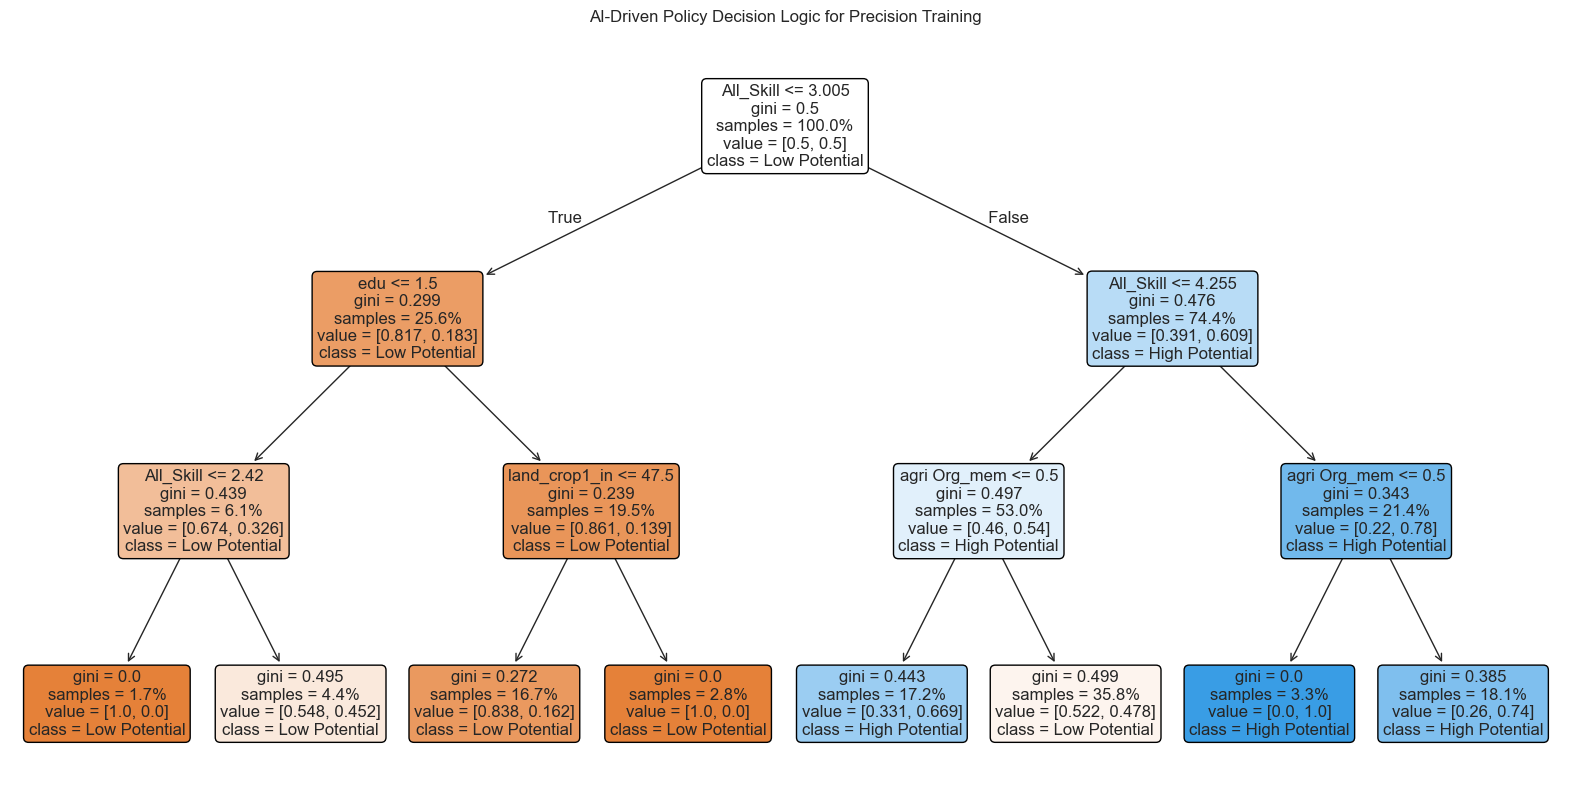
\includegraphics[width=0.9\textwidth]{images/fig_decisionTree.png}
\caption{กรอบการสังเคราะห์ผลการประเมินโครงการ: การบูรณาการผลเชิงสาเหตุ (PSM-DID) และผลเชิงพยากรณ์ (Machine Learning/SHAP) ร่วมกับการจำแนกกลุ่ม เพื่อนำไปสู่ข้อเสนอเชิงนโยบายแบบจำเพาะกลุ่ม}
\label{fig:synthesis}
\end{figure}

โดยสรุป ภาพที่~\ref{fig:synthesis} สะท้อนแนวทางการตีความผลการวิจัยแบบบูรณาการ กล่าวคือ ใช้ DID เป็นแกนกลางในการประเมินผลกระทบเชิงสาเหตุในระดับค่าเฉลี่ย ขณะที่ผลจาก Machine Learning/SHAP และการจัดกลุ่มถูกใช้เพื่อทำความเข้าใจความแตกต่างในระดับรายบุคคล

เมื่อพิจารณาภาพรวมของหลักฐานทั้งหมดร่วมกัน ผลการวิเคราะห์สะท้อนว่า การยกระดับทักษะขึ้นอยู่กับทั้งความพร้อมตั้งต้นและข้อจำกัดเชิงโครงสร้างของเกษตรกร

ดังนั้น การออกแบบนโยบายจึงควรหลีกเลี่ยงการใช้แนวทางแบบ one-size-fits-all และควรมุ่งเน้นมาตรการแบบจำเพาะกลุ่มเพื่อเพิ่มประสิทธิภาพของการพัฒนาทักษะในภาพรวม

\section{ข้อจำกัดของการศึกษา (Limitations)}

ตามที่สังเคราะห์ในหัวข้อ 4.9 การตีความผลการประเมินโครงการควรพิจารณาควบคู่กับข้อจำกัดของข้อมูล วิธีวิจัย และกรอบการอนุมาน โดยเฉพาะประเด็นที่อาจมีผลต่อความเที่ยงตรงเชิงสาเหตุของค่าประมาณจาก PSM/DID และขอบเขตการตีความผลจากการวิเคราะห์เชิงพยากรณ์ (machine learning/SHAP)

ดังนั้น หัวข้อนี้จึงสรุปข้อจำกัดสำคัญเพื่อประกอบการตีความผลการศึกษาอย่างรอบคอบ ดังต่อไปนี้

\begin{itemize}

\item \textbf{สมมติฐานแนวโน้มขนานของ DID (parallel trends assumption):} แม้หลักฐานเชิงกราฟในภาพที่~\ref{fig:parallel} สนับสนุนแนวโน้มขนานในช่วงก่อนโครงการ แต่ยังไม่อาจตัดความเป็นไปได้ของปัจจัยภายนอกที่ส่งผลแตกต่างกันระหว่างกลุ่มในช่วงเวลาศึกษา เช่น สภาพอากาศสุดขั้ว ราคาสินค้าเกษตร หรือมาตรการภาครัฐอื่น ซึ่งอาจทำให้ค่าประมาณ DID มีความเอนเอียง

\item \textbf{อคติจากการคัดเลือกและปัจจัยไม่สังเกตได้ (selection bias from self-selection/unobserved confounding):} วิธี PSM ช่วยลด selection bias ได้เฉพาะส่วนที่อธิบายได้ด้วยตัวแปรร่วมที่สังเกตได้ (selection on observables) จึงยังอาจมีปัจจัยที่ไม่ถูกวัด เช่น แรงจูงใจ เครือข่ายทางสังคม หรือความสามารถในการเรียนรู้ ที่สัมพันธ์ทั้งกับการเข้าร่วมโครงการและผลลัพธ์ ส่งผลให้ค่าประมาณ DID อาจมีความเอนเอียง

\item \textbf{ความคลาดเคลื่อนในการวัดผลและข้อจำกัดของดัชนีทักษะ (measurement error/index limitation):} หากตัวชี้วัดทักษะมีความไวต่อการเปลี่ยนแปลงต่ำ มีเพดานคะแนน (ceiling effect) หรืออาศัยการรายงานตนเอง อาจทำให้ตรวจไม่พบผลกระทบแม้มีการเปลี่ยนแปลงเกิดขึ้นจริง

\item \textbf{ช่วงเวลาศึกษาและความเข้มข้นของการดำเนินโครงการ (time horizon/program intensity):} การประเมินผลใช้ข้อมูลก่อน–หลังเพียงสองช่วงเวลา (ปี 2565–2566) อาจยังไม่เพียงพอต่อการจับผลลัพธ์ที่เกิดช้า (lagged effects) อีกทั้งความเข้มข้นของกิจกรรมอาจแตกต่างกันระหว่างพื้นที่ ทำให้ผลกระทบเฉลี่ยถูกลดทอน

\item \textbf{ขอบเขตการตีความผลจากการวิเคราะห์เชิงพยากรณ์ (machine learning/SHAP interpretation):} ผลการวิเคราะห์ส่วนนี้สะท้อนความสัมพันธ์เชิงพยากรณ์และความไม่เป็นเนื้อเดียวกันของข้อมูล (heterogeneity) ไม่สามารถตีความเป็นเหตุและผลโดยตรง และอาจไวต่อการเลือกตัวแปร การตั้งค่าของแบบจำลอง และโครงสร้างข้อมูลที่ใช้ฝึกแบบจำลอง

\item \textbf{ขอบเขตการอ้างอิงทั่วไปของผลการศึกษา (external validity):} ผลการศึกษานี้อ้างอิงจากกลุ่มตัวอย่างและบริบทพื้นที่ตามข้อมูลที่มีอยู่ จึงควรระมัดระวังในการขยายผลไปยังพื้นที่หรือกลุ่มเกษตรกรที่มีโครงสร้างการผลิต ทรัพยากร และสภาพแวดล้อมเชิงนโยบายแตกต่างกัน

\end{itemize}